%% by Michael Shell
%% Edited by Rodrigo Almeida
%%
%% This work is distributed under the LaTeX Project Public License (LPPL)
%% ( http://www.latex-project.org/ ) version 1.3, and may be freely used,
%% distributed and modified. A copy of the LPPL, version 1.3, is included
%% in the base LaTeX documentation of all distributions of LaTeX released
%% 2003/12/01 or later.
%% Retain all contribution notices and credits.

\documentclass[10pt,journal,compsoc]{IEEEtran}

\hyphenation{op-tical net-works semi-conduc-tor}

\usepackage{hyperref}
\usepackage{biblatex}
\usepackage{graphicx}
\usepackage{listings}
\usepackage{multirow}
\usepackage{tabularx}
\usepackage{caption}
\usepackage{booktabs}
\usepackage{xcolor}
\usepackage{float}

% Define custom colors for syntax highlighting (optional)
\definecolor{codegreen}{rgb}{0,0.6,0}
\definecolor{codegray}{rgb}{0.5,0.5,0.5}
\definecolor{codepurple}{rgb}{0.58,0,0.82}
\definecolor{backcolour}{rgb}{0.95,0.95,0.92}

\lstset{
    language=Python,
    caption={Training a Decision Tree Classifier},
    captionpos=b,
    basicstyle=\scriptsize, % Adjust the font size here
    backgroundcolor=\color{backcolour}, % Background color (optional)
    commentstyle=\color{codegreen},
    keywordstyle=\color{blue},
    numberstyle=\tiny\color{codegray},
    stringstyle=\color{codepurple},
    breakatwhitespace=false,
    breaklines=true,
    numbers=left,
    showstringspaces=false,
    showtabs=false,
    tabsize=1,
    frame=none,
    linewidth=0.95\columnwidth, % Adjust the line width to fit within the column
    xleftmargin=0.05\columnwidth,
}

\graphicspath{{images/}}

\addbibresource{references.bib}

\begin{document}
% paper title
% Titles are generally capitalized except for words such as a, an, and, as,
% at, but, by, for, in, nor, of, on, or, the, to and up, which are usually
% not capitalized unless they are the first or last word of the title.
% Linebreaks \\ can be used within to get better formatting as desired.
% Do not put math or special symbols in the title.
% \title{Transparency in AI - Decision-Making with Explainable AI (XAI)}
\title{Why Explain a decision made by AI? Explainable AI (XAI)}

% author name
\author{Rodrigo Almeida% <-this % stops a space
}

% The paper headers
\markboth{Research Methods in Computing \& IT - Literature Review}%
{}

\IEEEtitleabstractindextext{
    \begin{abstract}
        This paper will review the literature on transparency for artificial intelligence (AI) decisions. As AI advances, our dependence on AI models increases, 
        and the need to understand the model that made such a decision becomes more critical.
         Explainable Artificial Intelligence (XAI) has become an excellent choice due to the complexity of AI, 
        explaining the outputs with more clarity and transparency to the decision-making process, as opposed to "Black Box" algorithms that cannot explain why or how the AI 
        arrived in a conclusion, outputting directly from data, and not even who developed such algorithms can explain how the model arrived in such a result.
    \end{abstract}
}

% make the title area
\maketitle

\section{Introduction}
\label{sec:introduction}


\IEEEPARstart{A}rtificial intelligence is increasingly becoming a part of everyday life, being used in critical applications, from healthcare to finance and even in the military sector, 
whether it is to help with medical diagnoses, self-driving cars or even to help with the decision-making process in the military sector.
As AI advances, our dependence on AI models increases, and the need to understand the model that made such a decision becomes more critical.
As a result, there is a growing need for AI systems to be more than just accurate and efficient. They must also be transparent, interpretable, and explainable. 
This is particularly important for critical applications where the consequences of a wrong prediction can be severe. \cite{transparency}
Decisions made by AI systems can significantly impact people's lives, and it is essential to understand how these decisions are made.\cite{analytical-review} 
It is not only a technical challenge but also a social one. The general public, policymakers, and regulators are increasingly concerned about the impact of AI systems on society. \cite{doshivelez2017rigorous}
The impact of the outcome will vary based on the field. A wrong prediction for computing and business might lead to misleading recommendations, potentially affecting the revenue of such businesses. 
However, wrong predictions in critical sectors like healthcare could risk human life. Opening the "black box" is incredibly important, not just for social acceptance but also for regulatory purposes. 
Understanding how AI systems reach their conclusions is crucial in ensuring accountability, transparency, and ethical use of these technologies, making it essential for both public trust and regulatory compliance.\cite{analytical-review}


In \autoref{fig:xaiGraphic}, we can easily understand the main differences between the "Black Box" and XAI.\cite{xai-concept}

\begin{figure}[h]
    \centering
    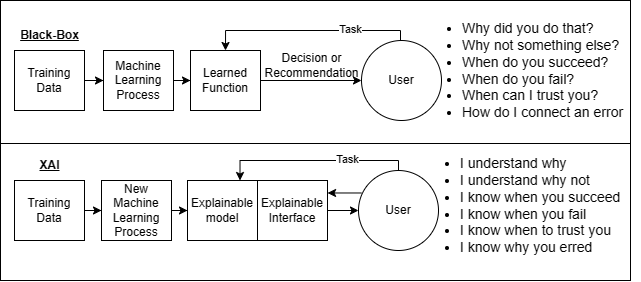
\includegraphics[scale=0.37]{images/xaiGraphic.png}
    \caption{Black box vs XAI}
    \label{fig:xaiGraphic}
\end{figure}

\section{Definitions}

Explainable AI (XAI) is a field focused on increasing human understanding of AI systems. Although terms like transparency, interpretability, and explainability are frequently used together, they can have different meanings, and there are differences between these theories.\cite{antoniadi2021current}

\begin{itemize}
    \item {Transparency}: a model deemed transparent can be understood easily on its own. It is the opposite of a "black box", indicating that the models's inner workings are understandable\cite{transparency}.
    \item {Interpretability}: It is the ability to explain complex concepts or results in a way humans can easily understand\cite{gilpin2019explaining}.
    \item {Explainability}: the concept that provides explanations as a bridge between AI systems and humans. It involves the ability to create AI systems that are not only accurate but also that people can understand.\cite{gilpin2019explaining}.
\end{itemize}

\section{Overview of Explainable AI Algorithms}
Researchers have developed many algorithms to explain AI systems. These explanations could be categorized into two primary groups: self-interpretable models refer to the algorithm model itself or a representation of the algorithm that can be directly read and comprehended by a human. In this case, the model itself serves as the explanation. On the other hand, post-hoc explanations are descriptions, explanations, or models of the algorithm often produced by separate software tools. These tools aim to provide an understanding of how the algorithm operates. Post-hoc explanations are handy for algorithms whose inner workings are not entirely transparent, as they can be employed to generate insights without requiring deep knowledge of the algorithm's internal mechanisms. Instead, they rely on querying the algorithm for outputs based on selected inputs.\cite{phillips2020four}.

\subsection{Self-interpretable Models}
Models that are self-interpretable are those that serve as the explanation themselves. They not only describe the entire model but also go through each input, replicating it on the self-interpretable model, justifying each decision.
Common self-interpretable models are decision trees and regression models. Ongoing research aims to create more interpretable models that surpass the accuracy of basic decision trees and regression models. These newer models include decision lists, decision sets, prototypes (representative samples of each class), feature combination rules, Bayesian Rule Lists, additive decision trees, and improved versions of decision trees.\cite{phillips2020four}
Some sources suggest a trade-off between accuracy and interpretability, with self-interpretable models being less accurate than post-hoc models. In this case, the challenge is to balance the precision of the model with what it means to humans. However, scholars like Rudin\cite{rudin} and Radin\cite{radin}, in their research called "Why Are We Using Black Box Models in AI When We Don’t Need To? A Lesson From an Explainable AI Competition", disagree, 
explaining that a trade-off between accuracy and interpretability is not always necessary. They argue that interpretable models can be used without sacrificing accuracy. \cite{phillips2020four}

\subsection{Pos-hoc Explanations}
Post-hoc explanations refer to an explanation given after a model has been trained. In other words, the explanations are generated after the model has made the decision or prediction and not during the training phase. It is divided into two: local explanation and global explanation.

\subsection{Local Explanation} Local explanations explain a subset of inputs. It focuses on explaining the output for a specific data point. The most common type is a per-decision or single-decision explanation, which explains the output or decision on a single input.\cite{phillips2020four}
These explanations focus on a single prediction and aim to answer the following question: "Why did this model make that particular prediction for that specific task?" There are some techniques used for local explanation. Some of the techniques used for local explanation are:

\subsubsection{LIME - Local Interpretable Model-agnostic Explainer}
LIME takes a specific decision made by an ML model and examines nearby data points, creating a simplified and interpretable model representing a locally made decision\cite{phillips2020four}. The default model is logistic regression.
LIME breaks down the image into smaller regions called superpixels when dealing with images. It then explores combinations of these superpixels, omitting some and replacing some with black. By doing this, LIME aims to understand and explain how the model's decision is influenced by specific parts of the image.

\subsubsection{SHAP - SHapley Additive exPlanations} SHAP is based on game theory concepts and can explain the predictions by calculating the contribution of every feature to the prediction. It explains how each feature impacts every model's prediction by considering their interaction consistently and fairly. This helps increase the interpretability by explaining the logic behind every prediction.\cite{why-trust-you}

\subsection{Global Explanations}
Global explanations produce post-hoc explanations throughout the whole dataset. It outlines the process used for the decision-making, mentioning tendencies,\\
features and possible biases that the model should have learned from the data. Global explanations are essential to understanding the model's behaviours and ensuring fairness, identifying biases, and increasing trust in AI systems. \\
Such context in XAI helps stakeholders cope with potential issues by understanding the impact and implications of decisions made by a model. Some of the techniques used for global explanation are:

\subsubsection{PDPs - Partial Dependence Plots}
PDPs show the change in the response when a value changes in the feature, showing the relationship between the feature and the response. It is a global method, meaning that it considers all the data points in the dataset.
The advantage of PDPs is that it is easy to understand and can be used for any model. Especially useful when trying to understand the relationship between a feature and the response and how the model behaves for individual features.\cite{phillips2020four}

\subsubsection{ICE - Individual Conditional Expectation Curves}
Individual conditional expectation curves are a more user-friendly way to understand how a feature influences a prediction for a single instance, by doing so, it makes it easier to understand how the model behaves for a specific case.

\subsubsection{TCAV - Testing with Concept Activation Vectors}
This is a global algorithm designed to explain neural networks in a way that is easier to understand. It represents the neural network state using a linear interpretation of the internals of deep learning.

\subsubsection{CAVs - Concept Activation Vectors}
Concept Activation Vectors are user-friendly concepts used by TCAVs to explain neural networks. It is the numerical representation of a concept, making it more understandable to humans.

\subsubsection{Decision sets}
Unlike black-box models, decision sets capture the decision-making process by generating a set of rules outlining the conditions in which the model predicts specific outcomes, helping understand the model's decision boundaries.

\begin{table}[H]
    \centering
    \small
    \begin{tabularx}{\columnwidth}{|p{1.8cm}|X|X|}
        \hline
        \textbf{Aspect}           & \textbf{Local Explanation}                                                                                              & \textbf{Global Explanation}                                                                                                                                    \\
        \hline
        \textbf{Scope}            & It explains individual predictions.                                                                                     & It will focus on understanding the model's behaviour across the entire dataset.                                                                                \\
        \hline
        \textbf{Granularity}      & Aims to explain why a particular decision was made.                                                                     & Higher level overview of the model's behaviour, bringing up general trends and feature importance across the dataset.                                          \\
        \hline
        \textbf{Techniques}       & LIME, SHAP, individual instance inspection.                                                                             & PDPs, ICE, SP-LIME, TCAV, decision sets, and summary of counterfactual rules.\cite{phillips2020four}                                                               \\
        \hline
        \textbf{Use Cases}        & Focus on explaining why a specific prediction was made, especially in critical applications like healthcare or finance. & Focus on identifying biases, ensuring fairness, and gaining an overall understanding of the model's behaviour for regulatory compliance and model improvement. \\
        \hline
        \textbf{Interpretability} & Easier to understand individual cases focusing on the specific explanation.                                        & A wider view of the model makes it valuable for stakeholders and policymakers seeking a general understanding of the AI system.                                \\
        \hline
    \end{tabularx}
    \caption{Comparison of Local and Global Explanations in XAI}
    \label{tab:xai_comparison}
\end{table}

\section{Interpreting Predictions - A Case Study with the "Adult Income" dataset}
As a case study, I will use the "Adult Income" dataset\cite{misc_adult_2} to predict whether an individual earns more than €50,000/year based on 14 features. This dataset was extracted by Barry Becker \cite{misc_adult_2} and is often cited in machine learning literature and research papers.
Table \ref{tab:variable-descriptions} shows the 14 features listed by name, role type and demographic.

\begin{table}[h]
    \centering
    \caption{Variable Descriptions}
    \begin{tabularx}{\columnwidth}{cccccc}
        \toprule
        \textbf{Variable Name} & \textbf{Role} & \textbf{Type} & \textbf{Demographic} \\
        \midrule
        age                    & Feature       & Integer       & Age                  \\
        work class              & Feature       & Categorical   & Income               \\
        fnlwgt                 & Feature       & Integer       & ---                  \\
        education              & Feature       & Categorical   & Education Level      \\
        education-num          & Feature       & Integer       & Education Level      \\
        marital-status         & Feature       & Categorical   & Other                \\
        occupation             & Feature       & Categorical   & Other                \\
        relationship           & Feature       & Categorical   & Other                \\
        race                   & Feature       & Categorical   & Race                 \\
        sex                    & Feature       & Binary        & Sex                  \\
        capital-gain           & Feature       & Integer       & ---                  \\
        capital-loss           & Feature       & Integer       & ---                  \\
        hours-per-week         & Feature       & Integer       & ---                  \\
        native-country         & Feature       & Categorical   & Other                \\
        income                 & Target        & Binary        & Income               \\
        \bottomrule
    \end{tabularx}
    \label{tab:variable-descriptions}
\end{table}

\begin{itemize}
    \item \textbf{Age:} It represents the age of a person, it is an important factor in predicting income because age can reflect an individual's level of experience and earning potential.

    \item \textbf{Work class:} It can be categorized as Private, Self-emp-not-inc, Self-emp-inc, Federal-gov, Local-gov, State-gov, Without-pay, Never-worked. It refers to the type of employment. Employment status is also essential, as income levels often vary according to employment status.

    \item \textbf{Fnlwgt:} Final weight represents the number of people the census believes the entry represents.

    \item \textbf{Education Level:} Represents the highest level of education an individual has obtained. It is divided into Bachelors, Some-college, 11th, HS-grad, Prof-school, Assoc-acdm, Assoc-voc, 9th, 7th-8th, 12th, Masters, 1st-4th, 10th, Doctorate, 5th-6th, Preschool. The education level is a key predictor of income since individuals with higher education often have access to better-paying job opportunities.

    \item \textbf{Education Num:} This is a numerical representation of the educational level. This also helps understand the education obtained by an individual.

    \item \textbf{Marital Status:} This describes the marital status of the individual. It is divided into Married-civ-spouse, Divorced, Never-married, Separated, Widowed, Married-spouse-absent, and Married-AF-spouse.

    \item \textbf{Occupation:} Specifies the type of education the individual is involved with. It is divided into Tech-support, Craft-repair, Other-service, Sales, Exec-managerial, Prof-specialty, Handlers-cleaners, Machine-op-inspct, Adm-clerical, Farming-fishing, Transport-moving, Priv-house-serv, Protective-serv, Armed-Forces. Occupation is also a critical factor that influences income, as income levels are different depending on occupation.

    \item \textbf{Relationship:} This describes the relationship status of an individual, which can have an impact on household income and financial stability. It is divided into Wife, Own-child, Husband, Not-in-family, Other-relative, and Unmarried.

    \item \textbf{Race:} Indicates the race of the individual. It should not directly affect income but could be linked to other socioeconomic factors that can impact earnings. It is divided into White, Asian-Pac-Islander, Amer-Indian-Eskimo, Other, and Black.

    \item \textbf{Sex:} Specifies the gender of the individual. It can influence income for reasons such as wage gaps and job segregation. It is divided into females and males.

    \item \textbf{Capital Gain:} Represents capital gains for the individual. It contributes to overall income.

    \item \textbf{Capital Loss:} Represents capital losses for the individual. It can impact the individual's financial situation.

    \item \textbf{Hours Per Week:} Indicates the number of working hours per week. The number of hours worked in a week influences the income directly.

    \item \textbf{Native Country:} Indicates the individual's country of origin. Depending on the country of origin, the individual may be impacted by fewer or more opportunities. It is divided into United-States, Cambodia, England, Puerto-Rico, Canada, Germany, Outlying-US(Guam-USVI-etc), India, Japan, Greece, South, China, Cuba, Iran, Honduras, Philippines, Italy, Poland, Jamaica, Vietnam, Mexico, Portugal, Ireland, France, Dominican-Republic, Laos, Ecuador, Taiwan, Haiti, Columbia, Hungary, Guatemala, Nicaragua, Scotland, Thailand, Yugoslavia, El-Salvador, Trinadad \& Tobago, Peru, Hong, Holand-Netherlands.

    \item \textbf{Income:} This is the target variable indicating whether the individual's income exceeds  \$50,000 per year. \textbf{This is the variable we are trying to predict}.

\end{itemize}

\subsection{Using Python to Interpret Predictions}
In this section, the predictions made by a machine learning model using the "Adult Income" dataset will be interpreted using Python. Library \texttt{pandas} will be used for data handling, \texttt{sklearn} for building the model, and \texttt{shap} and \texttt{lime} for explainability.

\subsubsection{Loading and Preparing the Dataset}
Using Panda, the first step is to load the data and preprocess it in a way that handles missing values and splits the dataset into features \texttt{X} and target \texttt{y}.

\subsubsection{Training a Machine Learning Model}
To train the model, \texttt{DecisionTreeClassifier} from scikit-learn will be used for the classification task. The model will be trained using the training set and then used to make predictions on the test set.

\begin{lstlisting}[caption=Training a Decision Tree Classifier]
    # Train the Model
    decision_tree_model = DecisionTreeClassifier(random_state=42)
    decision_tree_model.fit(X_train, y_train)
    # Make predictions
    y_pred = decision_tree_model.predict(X_test)
\end{lstlisting}

\subsubsection{Evaluating the Model}
To evaluate the model, I will be using the \texttt{accuracy\_score} from scikit-learn. The accuracy score is the fraction of predictions the model got right.

\begin{lstlisting}[caption=Evaluating the Model]
    # Evaluate the classifier
    accuracy = accuracy_score(y_test, y_pred)
    print(f"Decision Tree Accuracy: {accuracy}")
\end{lstlisting}

\texttt{accuracy\_score} returns the accuracy of the model, which is 0.81, meaning that the model got 81\% of the predictions right.

\subsubsection{Global Explanation with Feature Importance
}

To understand the overall model behaviour, we can use the feature importance to understand which features are more critical for the model. The higher the value, the more important the feature is for the model.

\begin{lstlisting}[caption=Feature Importance, label=feature_importances]
    # Get feature importance
    importance = model.feature_importances_
    # Plot feature importance
    plt.barh(X.columns, importance)
    plt.xlabel("Feature Importance")
    plt.ylabel("Feature")
    plt.show()    
\end{lstlisting}

\begin{figure}[H]
    \centering
    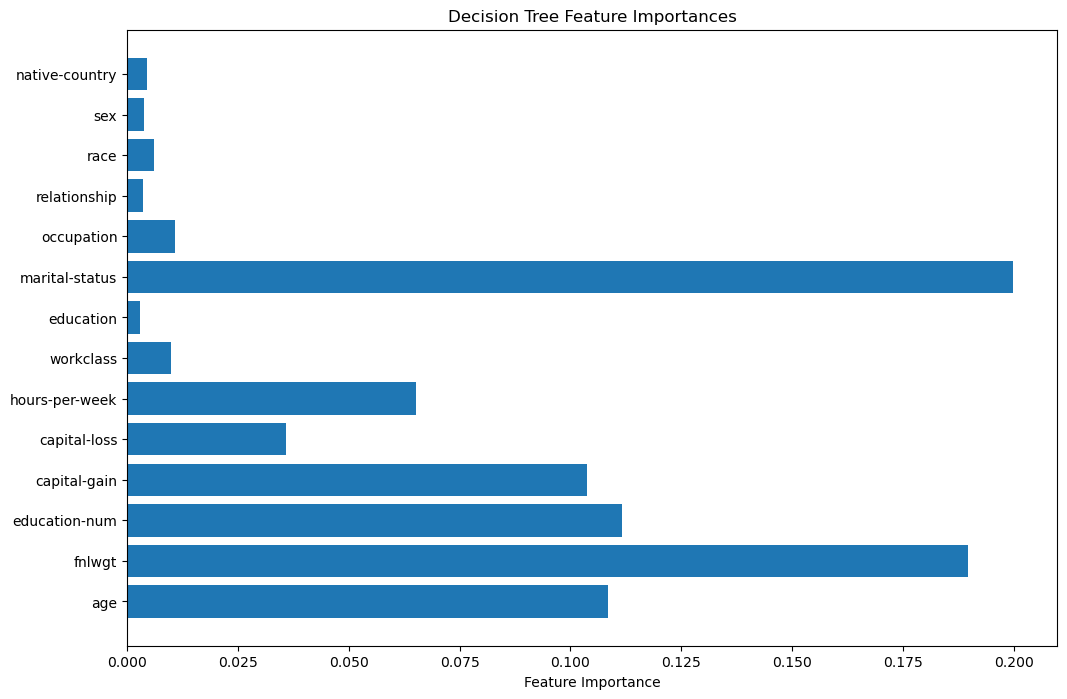
\includegraphics[width=1\linewidth]{images/feature_importance_global.png}    
    \caption{Decision Tree Feature Importance}
    \label{fig:feature_importances}
\end{figure}

\autoref{fig:feature_importances} shows the output of code from Listing~\ref{feature_importances} for the "Adult Income" dataset. We can see that the most important features are \texttt{marital-status}, \texttt{fnlwgt}, \texttt{education-num}, \texttt{age} and \texttt{capital-gain}.


\subsubsection{Local Explanation with SHAP}
I will first use SHAP (SHapley Additive exPlanations) for local explanations. It explains each feature, showing how each feature contributes to the prediction. 

\begin{lstlisting}[caption=SHAP Explainer , label=shap_explainer]
    shap_values = shap.TreeExplainer(decision_tree_model).shap_values(X)
    shap.summary_plot(shap_values, X)
\end{lstlisting}

\begin{figure}[H]
    \centering
    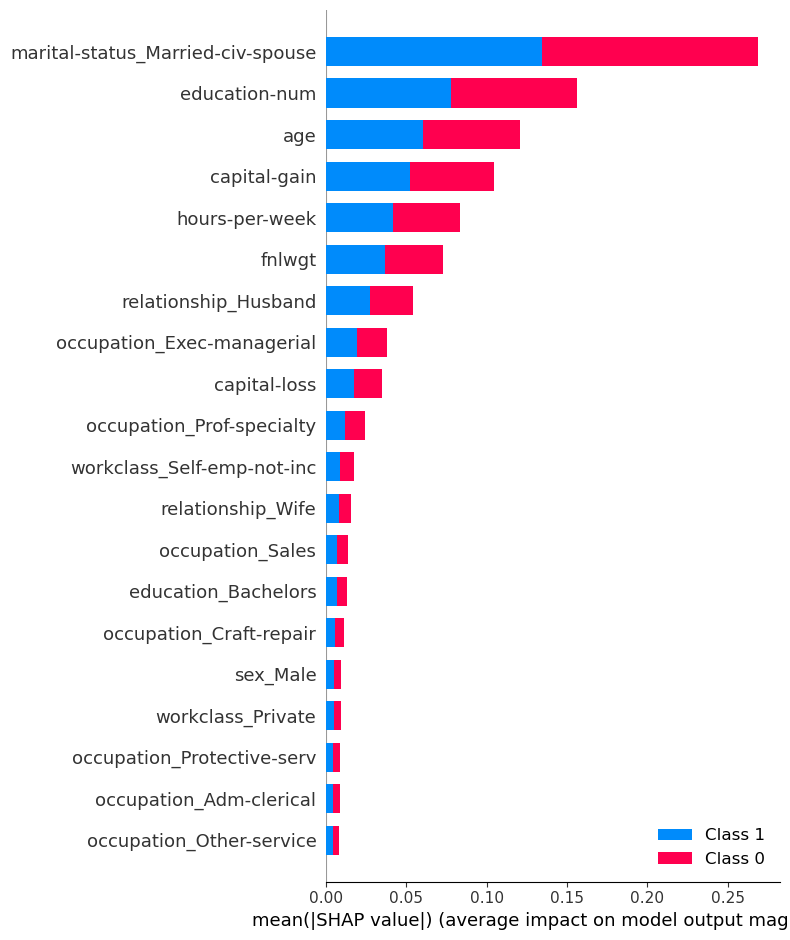
\includegraphics[width=1\linewidth]{images/shap_summary_plot.png}
    \caption{SHAP Decision Plot}
    \label{fig:shap_explainer}
\end{figure}
\textit{Note: In this SHAP summary plot, 'class 0' corresponds to incomes '$\leq$€50,000', and 'class 1' corresponds to incomes '$>$€50,000'.}
\\

\autoref{fig:shap_explainer} shows the output of code from Listing~\ref{shap_explainer} for the "Adult Income" dataset. It demonstrates the key features influencing the model's predictions for the higher income bracket (class 1).
The \texttt{marital-status} is shown as the feature with the highest mean SHAP value of 0.1345, suggesting a strong association between being married and predicting higher income.
Regarding educational background, \texttt{education-num} with a mean SHAP value of 0.0779 suggests a considerable influence, meaning that the higher the education level, the higher the income. Similarly, 
\texttt{age} of the individual, with a mean SHAP value of 0.0603, indicates that older individuals tend to fall into the higher income category according to the model.
Financial indicators like \texttt{capital-gain} with a mean SHAP of 0.0524, and \texttt{hours-per-week} with 0.0417 are also prominent.
The more an individual earns from the capital gains, the more likely they are to fall into the higher income category. Similarly, the more hours an individual works per week, the more likely they are to fall into the higher income category.
Other features like \texttt{fnlwgt}, \texttt{relationship\_Husband} and various occupational roles such as \texttt{occupation\_Exec-managerial}, \texttt{occupation\_Prof-specialty} have smaller but significant positive SHAP values, indicating that these features also contribute to the model's predictions for the higher income category.


\subsubsection{Local Explanation with LIME}

Another option that can be used is LIME (Local Interpretable Model-agnostic Explainer). It also explains each feature, showing how each feature contributes to the prediction.


\begin{lstlisting}[caption=LIME Explainer , label=lime_explainer]
    # Extracting feature names and weights from the LIME explainer
    feature_names, weights = zip(*exp.as_list())    
    # Convert to list
    feature_names = list(feature_names)
    weights = list(weights)    
    # Check the data format
    print("The feature names are:", feature_names)
    print("Weights:", weights)    
    # Creating a bar plot
    plt.figure(figsize=(8, 6))
    sns.barplot(x=weights, y=feature_names, palette='viridis')
    plt.title('Contribution of each feature to the Prediction')
    plt.xlabel('Weight')
    plt.ylabel('Feature')
    plt.show()
\end{lstlisting}

\begin{figure}[H]
    \centering
    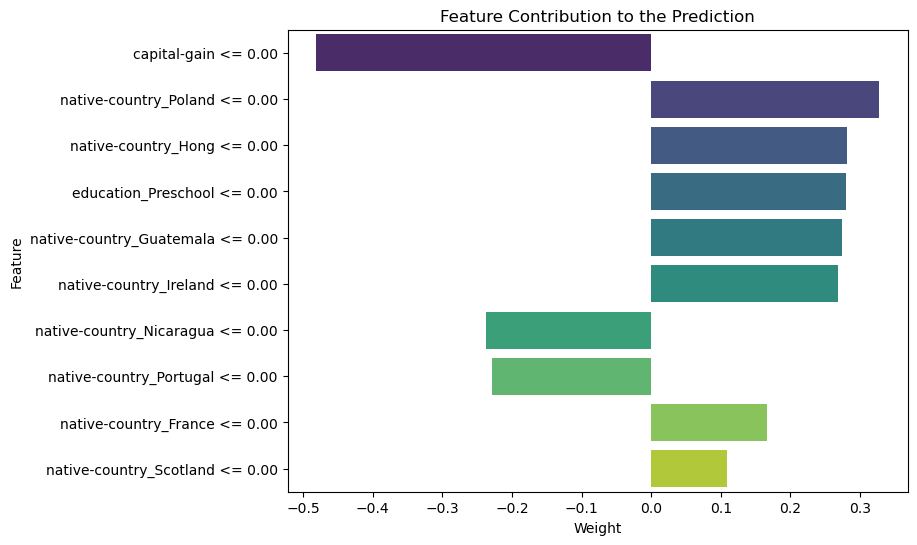
\includegraphics[width=1\linewidth]{images/lime_summary_plot.png}
    \caption{LIME Decision Plot}
    \label{fig:lime_explainer}
\end{figure}

\autoref{fig:lime_explainer} shows the output of the code from Listing~\ref{lime_explainer} for the "Adult Income" dataset. According to the model's prediction, this output highlights the top ten features that significantly influence an individual's income category.
Each feature is listed alongside a numerical weight, which quantifies the feature's influence on the prediction. 
The feature \texttt{capital-gain $\leq$ 0.00} has the most significant negative weight (-0.4817176518811231), suggesting that a strong link between having no or minimal capital gain and earning an income that is less than €50,000 annually. On the other hand, features such as \texttt{native-country\_Poland $\leq$ 0.00}, \texttt{native-country\_Hong $\leq$ 0.00}, and \texttt{education\_Preschool $\leq$ 0.00} has positive weights 
(0.3280648148846505, 0.2812235627400507, and 0.27962517534951975, respectively), suggesting that the absence of these conditions (e.g., not being from Poland, not being from Hong, not having preschool education) tends to be associated with earning a higher income. This LIME analysis provides a localized interpretation of a specific instance, offering insights into why the model might have predicted a particular income category for an individual based on their feature values. 
Other features, such as \texttt{native-country\_Guatemala $\leq$ 0.00} and \texttt{native-country\_Ireland $\leq$ 0.00}, also positively influence predictions towards a higher income, but their impact is somewhat less when compared to the other features. The negative weights of \texttt{native-country\_Nicaragua $\leq$ 0.00} 
and \texttt{native-country\_Portugal $\leq$ 0.00} indicates a tendency towards predicting lower income levels for individuals from these countries.


\section{Conclusion}
In conclusion, this literature review explored the importance of Explainable Artificial Intelligence (XAI), highlighting the importance of AI systems from various sectors, from healthcare to finance, to be more than just accurate and efficient.
They must also be transparent, interpretable, and explainable. This is particularly important for critical applications where the consequences of a wrong prediction can be severe. 
The review begins by addressing the challenges posed by the black box models that are difficult to explain and understand. It then discusses the importance of explainability in AI systems, highlighting the need for transparency, interpretability, and explainability.
The emergence of XAI is a response to these challenges, aiming to make AI decisions more transparent and interpretable. Diving into the core of XAI, the review differentiates between transparency, interpretability and explainability, highlighting the differences between these concepts.
Each of these aspects contributes uniquely to the goal of making AI more understandable and accountable.
Moreover, the case study using the "Adult Income" dataset demonstrates how XAI can be used to interpret predictions made by a machine learning model. Applying tools like SHAP and LIME provides insights into the model's behaviour, helping us understand why the model made a particular prediction for a specific individual.
This is particularly important for critical applications where the consequences of a wrong prediction can be severe.
AI is advancing rapidly and is becoming more integrated into our lives. As a result, the need for explainability will only increase. 
It is not only a technical challenge but also a social one. 
In summary, "Why Explain a Decision Made by AI?" is not only a question, but it is also a call to action for the AI community to make AI more transparent, interpretable, and explainable. The future of AI, as discussed in this review, is one where AI systems are not only accurate and efficient but also transparent, interpretable, and explainable, aligning with the needs of society, values and ethical considerations.



% references section
\printbibliography

\end{document}